%-----------------modello di sviluppo------------------------
\section{Ciclo di vita di un \Sw}
Abbiamo detto nell'introduzione che un processo di sviluppo di un \sw\ deve contenere le fasi fondamentali di: \textbf{specifica, sviluppo, convalida ed evoluzione.}
Compito del Ing del \Sw\ di regolare queste fasi del processo software quindi introdurre
un \textbf{Modello di processo}.
\begin{quote}
    Un \textbf{Modello di Processo} non \`e altro che la descrizione dell' ordine di esecuzione di queste attivit\`a, e stabilire quali sono i criteri da verificare per poi passare alla fase successiva.
    \label{quote:modello_di_processo}
\end{quote}
Quindi vogliamo utilizzare dei Modelli, che semplificano e soprattutto regola\-no il processo di sviluppo \sw \footnote{Il processo ovviamente dipende dal tipo di software, data la grande eterogeneit\`a dei \sw}.
\\
\subsection{Attivit\`a fondamentali nel ciclo di vita}
Introduciamo adesso le \textbf{Attivit\`a fondamentali} per lo sviluppo \sw .
\begin{itemize}
    \item \textbf{Studio di fattibilit\`a: }
        Fase che produce un documento con la definizione dei costi/benefici, i tempi di consegna e le modalit\`a di sviluppo
    \item \textbf{Specifica dei requisiti: }
        Fase che produce un documento che esplicita \textbf{COSA} il \sw\ dovr\`a fare e \textbf{NON COME}.
        quindi in questa fase non ci intressa la soluzione ma solo i requisiti.\footnote{Fase fondamanetale, errori in questa fase, corrompono tutte le successive. per torvarci infine un software che non soddisfa i requisiti del cliente}
        L'oggetto prodotto e' il \textbf{DSR} (Documento di specifica dei requisiti) ed eventualmente il \textbf{PTS} (Piano di test del sistema).
    \item \textbf{Progettazione: }
        Progettare una soluzione al problema. La progettazione avviene a vari livelli di dettaglio
        \begin{itemize}
            \item architettura generale: 
                (HW e SW)Quindi i vari componenti (moduli) utilizzati e la funzionalit\`a di ognuno
            \item architettura dettagliata: 
                descrizione dettagliata di ogni modulo.
                \footnote{Ad esempio in un approccio Client Server prima definiamo i moduli principali (client e server) poi andiamo nel dettaglio su ognuno.}
            \item DSP (documento di Progetto): 
                Documento che descrive i componenti (hw e sw) descrivendo il loro comportamento, le motivazioni delle scelte prese ed eventualemente future richieste.
        \end{itemize}
    \item \textbf{Produzione: }
        Implementazione effettiva della soluzione progettata, quindi comprende:
        \begin{itemize}
            \item codifica
            \item documentazione del codice
            \item testing del \sw
        \end{itemize}
    \item \textbf{Manutenzione: }
        Dopo il rilascio del \sw, lo sviluppo non \`e finito. Esistono i seguenti tipi di manutenzione del \sw :
        \begin{itemize}
            \item Correttiva: 
                correggere errori presenti nel codice, sfuggiti dalla fase di testing.
            \item Adattiva:
                addattare il nostro \sw\ ad un altra situazione (ad esempio nuovi S.O. , o cambio lingua).
            \item Perfettiva:
                Perfezionare il \sw, per migliorarne la qualit\`a (muntenibilit\`a, affidabilit\`a, efficienza e accetabilit\`a).
        \end{itemize}
\end{itemize}
%---------------------------MODELLI----------------------------------
\subsection{Modelli di Processo}
Abbiamo descritto nella pag. \pageref{quote:modello_di_processo}, la definizione di \textbf{Modello di Processo}. Ricapitolando, un modello di processo descrive l'ordine di esecuzione delle fasi fondamentali e i criteri da verificare alla fine di ogni fase.

Adesso introduciamo i principali modelli di processo pi\`u comuni.
In passato prima della creazione dell'ing del \sw\ si usava il metodo \textbf{Code And Fix}.

Consisiteva nel produrre codice e in seguito correggere gli errori presenti. \`E una soluzione primitiva,
non adatta a progetti di media/grande dimensione.
%--------------------WATERFALL-------------------------------------
\subsubsection{Modello a cascata: Waterfall}
Il modello \textbf{Waterfall} \`e il modello pi\`u semplice. Il concetto principale di questo modello \`e che ogni fase pu\`o essere eseguita solo alla fine della precedente.
Ogni fase alla sua fine, detta \textbf{Milestone}, produce un documento fondamentale per le fasi successive detto \textbf{deliverables}
, per questo motivo \`e detto \textbf{guidato dalla documentazione} (Approccio altamente burocratico).

Pu\`o essere descritto da tre aggettivi:
\begin{itemize}
    \item \textbf{Monoliticit\`a}: 
        Il progetto \`e completato solo alla fine di tutte le fasi
    \item \textbf{Rigidit\`a}:
        Si assume che i requisiti siano \textbf{Congelati} nella fase di specifica dei requisiti
    \item \textbf{Linerit\`a}:
        \`E lineare segue un modello di processo semplice, si parte da uno step se ne va in un altro. Non c'\`e parallelizzazione
\end{itemize}

\begin{figure}[htbp]
    \centering
    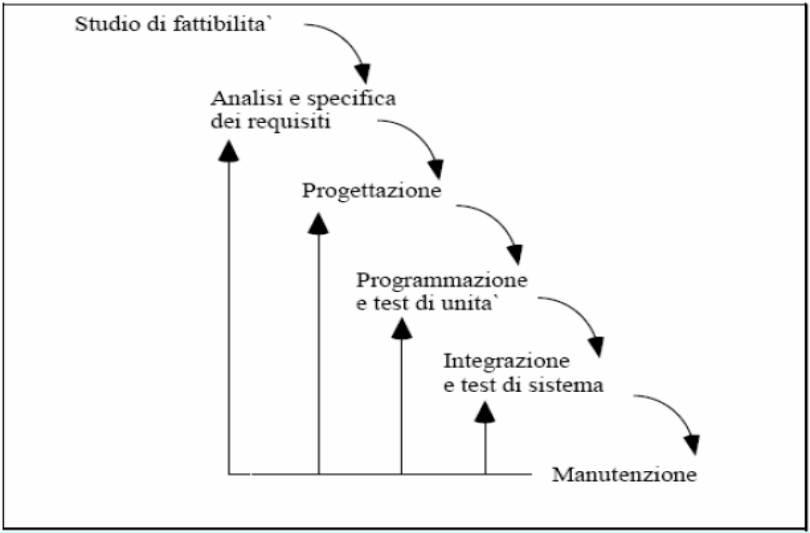
\includegraphics[scale=0.5]{cascata.PNG}
    \caption{Modello a Cascata}
    \label{fig:cascata}
\end{figure}
\newpage
Questo modello soffre di vari problemi tra cui:
\begin{itemize}
    \item \textbf{Suddivisione dei compiti:} 
        Si necessitano di figure che partecipano alle singole fasi, con il conseguente congelamento delle attivit\`a nei livelli sottostanti
    \item \textbf{Non modificabile: }
        Le modifiche nelle fasi successive, possono essere risolte solo alla terminazione, nella fase di manutenzione
    \item \textbf{Burocraticit\`a:} 
        Il modello dipende completamente dai documenti prodotti (i deliverables).
        Quindi rallentando di molto il processo
    \item \textbf{Stima dei costi:}
        \`E difficile effettuare una stima dei costi
    \item \textbf{Manutenzione:}
        Per la rigidit\`a, siamo obbligati ad una manutenzione frequente e sostanziosa, aumentando anche di molto il costo in termini economici e temporali.
\end{itemize}
\newpage
%--------------------FEEDBACK-------------------------------------
\subsubsection{Modello a Retroazione a Cascata}
\`E una variante del Modello Waterfall che introduce il concetto di \textbf{retroazione}.

Per retroazione indichiamo la possibilit\`a di poter \emph{tornare indietro}.
Quindi ad ogni fase introduciamo due ulteriori \textbf{sotto-fasi} quella di \textbf{convalida} e di \textbf{verifica}.
\begin{itemize}
    \item \textbf{Convalida:}
        Stabilire se il prodotto precedente \`e conforme alle sue specifiche
    \item \textbf{Verifica:}
        Verificare se il prodotto precedente \`e appropriato (\`e un parere {soggettivo}, non dipende dalle specifiche)
\end{itemize}
Per questo motivo \`e detto anche modello V \& V a feedback.

Sebbene risolve il problema della monoliticit\`a, del modello Waterfall, non pu\`o anticipare i cambiamenti. Quindi rimane sempre un modello lento, dovuto a questo overhead extra delle sotto-fasi di V \& V.
\begin{figure}[htpb]
    \centering
    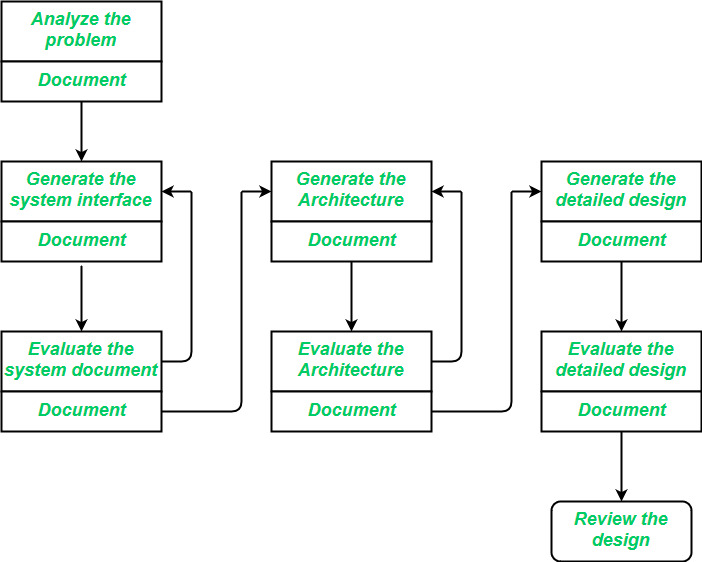
\includegraphics[scale=0.5]{feedback.jpg}
    \caption{modello V\&V a feedback}
    \label{fig:feedback}
\end{figure}
\newpage
%--------------------MODELLO A V---------------------------
\subsubsection{Modello a V}
Il modello a V, \`e ampiamente utilizzato nei \Sw\ dei sistemi \textbf{Embedded} e
nei sistemi di \textbf{controllo}.
\`E ampiamente basato sul \textbf{Testing}, in quanto \`e spesso richiesto un alto livello di affidabilit\`a.
Essendo un modello \textbf{testing driven}, \`e necessario un PTS (piano di testing).

\begin{figure}[htbp]
    \centering    
    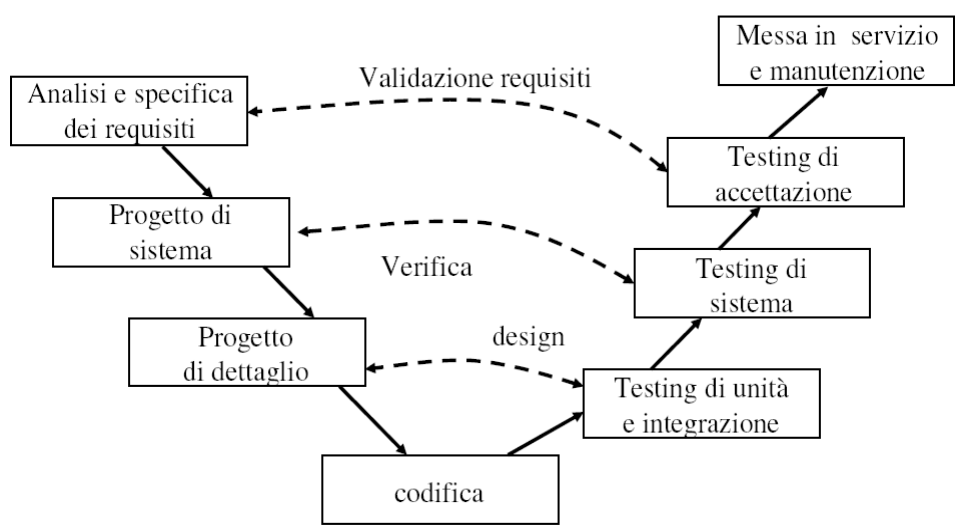
\includegraphics[scale=0.5]{modello_a_v.PNG}
    \caption{modello a V}
    \label{fig:modello a v}
\end{figure}    
Come vediamo dalla figura \`e un modello a doppia \textbf{retroazione}.
E notiamo che la validazione \`e l'errore pi\`u costoso, in quanto ci obbliga a tornare alla fase di analisi e specifica 
dei requisiti.

Particolare enfasi, in questo modello, viene data all'\textbf{Hardware}.

Come per il modello a cascata e la sua variazione (V \& V), viene usato per software in ambienti
poco soggetti a cambiamenti.
\subsection{Modelli Evolutivi}
i modelli evolutivi si basano sulla produzione di una versione iniziale (Prototipo),
questa versione verr\`a poi perfezionata attraverso varie versioni.
\subsubsection*{Prototipo}
\begin{quote}
    Un Prototipo \`e un modello dell' applicazione, il cui obbiettivo \`e quello di  ricevere feedback
    per affinare i requisiti.
\end{quote}
Quindi utilizziamo i prototipi per raccogliere feedback dagli stakeholders.
Questo permette un approccio pi\`u diretto col cliente, che diventa parte pi\`u integrante del progetto.
Cos\`i facendo miglioriamo i requisiti ed eventualmente li \textbf{completiamo}.

I modelli Evolutivi che si basano sui prototipi, si dividono in base al utilizzo di esso:
\begin{itemize}
    \item Prototipo \textbf{usa e getta}
    \item Prototipo \textbf{evolutivo}
\end{itemize}
\subsubsection{Sviluppo con prototipo usa e getta}
Con il prototipo usa e getta, si realizza una prima implementazione imperfetta e incompleta 
del \sw, con l'unico scopo di accertare la fattibilit\`a e validare i requisiti.
Poi il modello viene \textbf{gettato}.

Quindi si basa sul approccio ``\textbf{Do It Twice}``

Questo approccio \`e ampiamente utilizzato in \textbf{software house con una certa maturit\`a}. Questo perch\`e 
il prototipo \`e spesso creato con pezzi di codice gi\`a scritti, quindi \`e  facile e veloce realizzarne
uno.
\begin{figure}[htbp]
    \centering    
    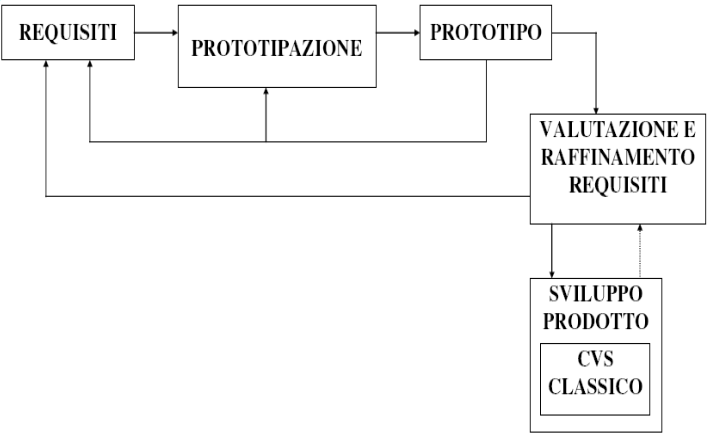
\includegraphics[scale=0.7]{modello_usa_e_gettta.PNG}
    \caption{modello prototipale usa e getta}
    \label{fig:prototipale usa e getta}
\end{figure}   
\\
La creazione del prototipo pu\`o avvenire in varie fasi, sia in quella di \textbf{specifica dei requisiti}
sia nella fase di \textbf{design}.
\newpage
\subsubsection{modello con prototipo evolutivo}
I modelli con prototipo evolutivo, a differenza dei modelli con prototipi ``usa e getta``, non gettano il prototipo
ma lo raffinano anche iterativamente, fino al prodotto finale.
\begin{figure}[htbp]
    \centering    
    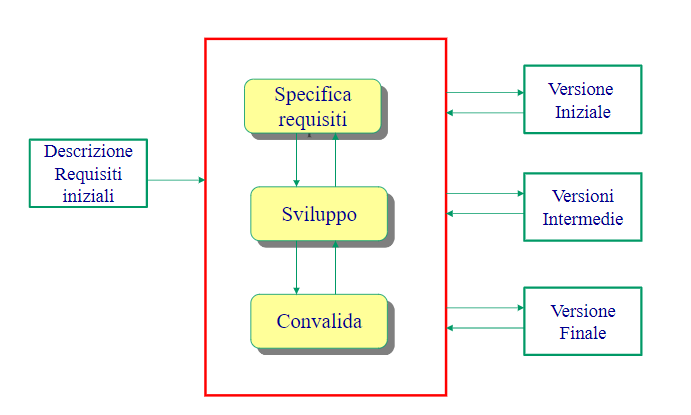
\includegraphics[scale=0.7]{modello_evolutivo.PNG}
    \caption{modello evolutivo}
    \label{fig:modello evolutivo}
\end{figure}   
\begin{itemize}
    \item vantaggi
        \begin{itemize}
            \item sviluppo veloce
            \item molti feedback dal cliente
            \item cambio dei requisiti pi\`u veloce
        \end{itemize}
    \item svantaggi
        \begin{itemize}
            \item minor qualit\`a dovuta al rattoppare il prototipo
            \item pessima documentazione o assente
            \item si necessit\`a di programmatori con esperienza in linguaggi di prototipazione
        \end{itemize}
\end{itemize}
\subsection{Modello incrementale}
Il modello incrementale, si basa sul rilascio ad \textbf{incrementi}.

Quindi il \sw\ non \`e rilasciato al completamento del \sw\ con tutti i requisiti soddisfatti
, ma si rilascia ad incrementi, cio\`e a \textbf{step}.
\begin{figure}[htbp]
    \centering    
    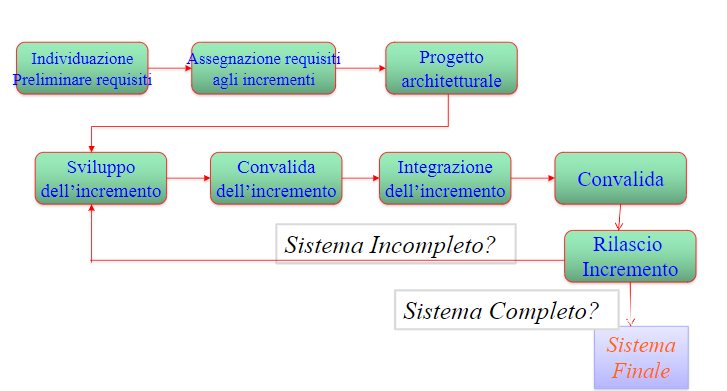
\includegraphics[scale=0.7]{modello_incrementale.PNG}
    \caption{modello incrementale}
    \label{fig:modello incrementale}
\end{figure}  
Quindi si associano dei livelli di \textbf{priorit\`a} ai vari requisiti
, e si sviluppano prima gli incrementi relativi a quelli con priorit\`a maggiore.

I primi incrementi, fungono da veri e propri prototipi, che possono essere col tempo evoluti,

Tra i vantaggi abbiamo:
\begin{itemize}
    \item Il cliente vede prima i risultati, risultando pi\`u soddisfatto
    \item Si riduce il rischio di fallimento del intero progetto
    \item I servizi con priorit\`a maggiore vengono testati in maniera pi\`u accurata
\end{itemize}
Invece tra gli svantaggi:
\begin{itemize}
    \item Non pu\`o essere usato se si necessita di sistemi completi
    \item Difficolt\`a nel identificazione degli incrementi con priorit\`a maggiore
\end{itemize}
\subsection{Modello trasformazionale}
I modelli trasformazionali, si basano su specifiche e requisiti scritti in linguaggi di
alto livello, spesso di natura \textbf{algebrica matematica, insiemistica o con automi a stati finiti},
in questo modo tramite 
dei processi di trasformazione, modifichiamo questi requisiti astratti 
man mano in \textbf{Codice Eseguibile}.

\`E basato su due concetti fondamanetali: 
\begin{itemize}
    \item Prototipazione
    \item Formalizzazione
\end{itemize}
Poich\`e con questo modello, si usa un approccio molto formale, diventa difficile
produrre \sw\ di grandi dimensioni, ma risulta molto comodo, tranne per uno sforzo iniziale
, con l'utilizzo di \textbf{codice riusabile}.

Per questo si dice che si avvale della \textbf{storia dello sviluppo}.
Pu\`o avvalersi di strumenti software che automatizzano il processo di sviluppo (code generation).
\subsection{Modello a spirale}
il modello a spirale \`e un \textbf{Meta-modello}, quindi serve per definire altri modelli.

Fulcro di questo modello sono \`e la \textbf{gestione dei rischi}:
\begin{quote}
    ``Identificare, affrontare, ed eliminare i rischi prima che insorgano problemi seri o causa di 
    re-implementazioni costose``
\end{quote}
\begin{figure}[htbp]
    \centering    
    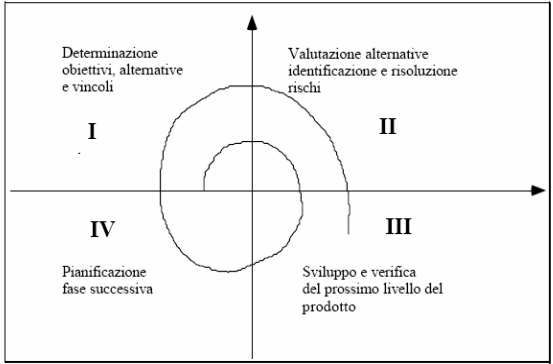
\includegraphics[scale=0.7]{modello_a_spirale.PNG}
    \caption{modello a spirale}
    \label{fig:modello a spirale}
\end{figure} 
come possiamo notare \`e suddiviso in quattro quadranti:
\begin{itemize}
    \item Determinazione obiettivi, alternative e vincoli:
    \item Valutazione alternative identificazione e risoluzione dei rischi
    \item Sviluppo e verifica del prossimo livello del prodotto
    \item Pianificazione fase succesiva
\end{itemize}
il \textbf{raggio} indica il costo accumulato, quindi \`e una spirale che cresce verso l'esterno.

\textbf{ATTENZIONE!!!} il modello a spirale \`e un meta-modello, quindi non esclude l'utilizzo
di altri modelli ad esempio un modello evolutivo o a cascata, a seconda dei requisiti.